\documentclass[CMPE]{KGCOEReport}
\usepackage{float}
\usepackage{adjustbox}
\graphicspath{ {./images/} }

\newcommand{\name}{Mohammed Fareed \\ Trent Wesley}
\newcommand{\exerciseNumber}{6}
\newcommand{\exerciseDescription}{Motor Control}
\newcommand{\dateDone}{October 18, 2023}
\newcommand{\dateSubmitted}{October 31, 2023}

\newcommand{\classCode}{CMPE 460}
\newcommand{\LabSectionNum}{1}
\newcommand{\LabInstructor}{Prof.\ Hussin Ketout}
\newcommand{\TAs}{Andrew Tevebaugh \\  Colin Vo}
\newcommand{\LectureSectionNum}{1}
\newcommand{\LectureInstructor}{Prof.\ Hussin Ketout}


\begin{document}
\maketitle

This laboratory exercise involved interfacing the MSP432 with a DC motor, a stepper motor, and a servo. First, the Timer A module was used to generate a PWM signal. Specifically, a 20\% duty cycle signal with a frequency of 10kHz was generated and viewed with an oscilloscope. Next, a DC motor was controlled. A SN754410 H-bridge IC was utilized to control the 10V power supply voltage with the 3.3V control voltage from the MSP432. The stepper motor was operated in full step, low torque mode by the MSP432 with a ULN2068B Darlington array IC. It was controlled by periodically switching which coils turned on based on the phase. The last type of motor tested was the servo motor. This was controlled by providing a 50Hz PWM signal with a pulse width between 1ms and 2ms. Finally, knowledge gained from testing these motors was used to control the servo and two DC motors on an MSP432-controlled miniature electric car.

\begin{figure}[H]
    \centering
    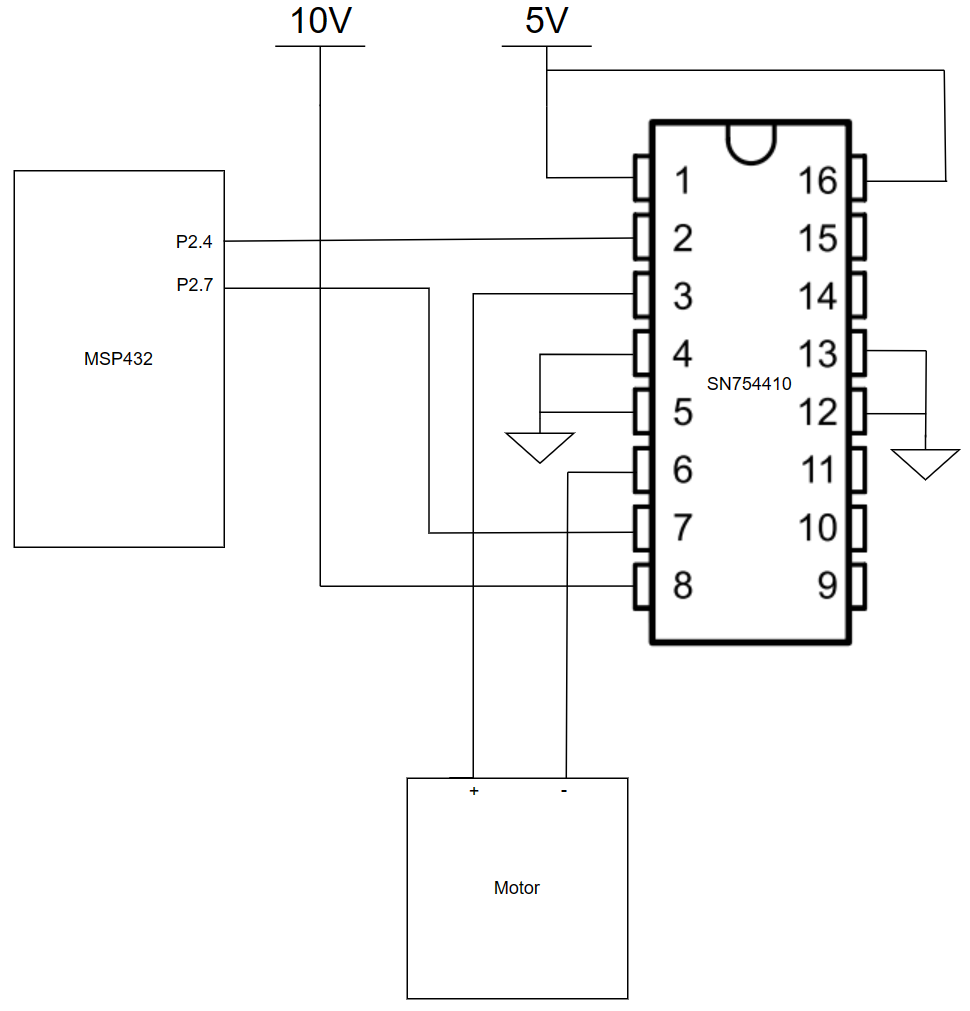
\includegraphics[width=0.75\textwidth]{DCMotorWiring.png}
    \caption{DC Motor Wiring}
    \label{fig:DCMotorWiring}
\end{figure}

\begin{figure}[H]
    \centering
    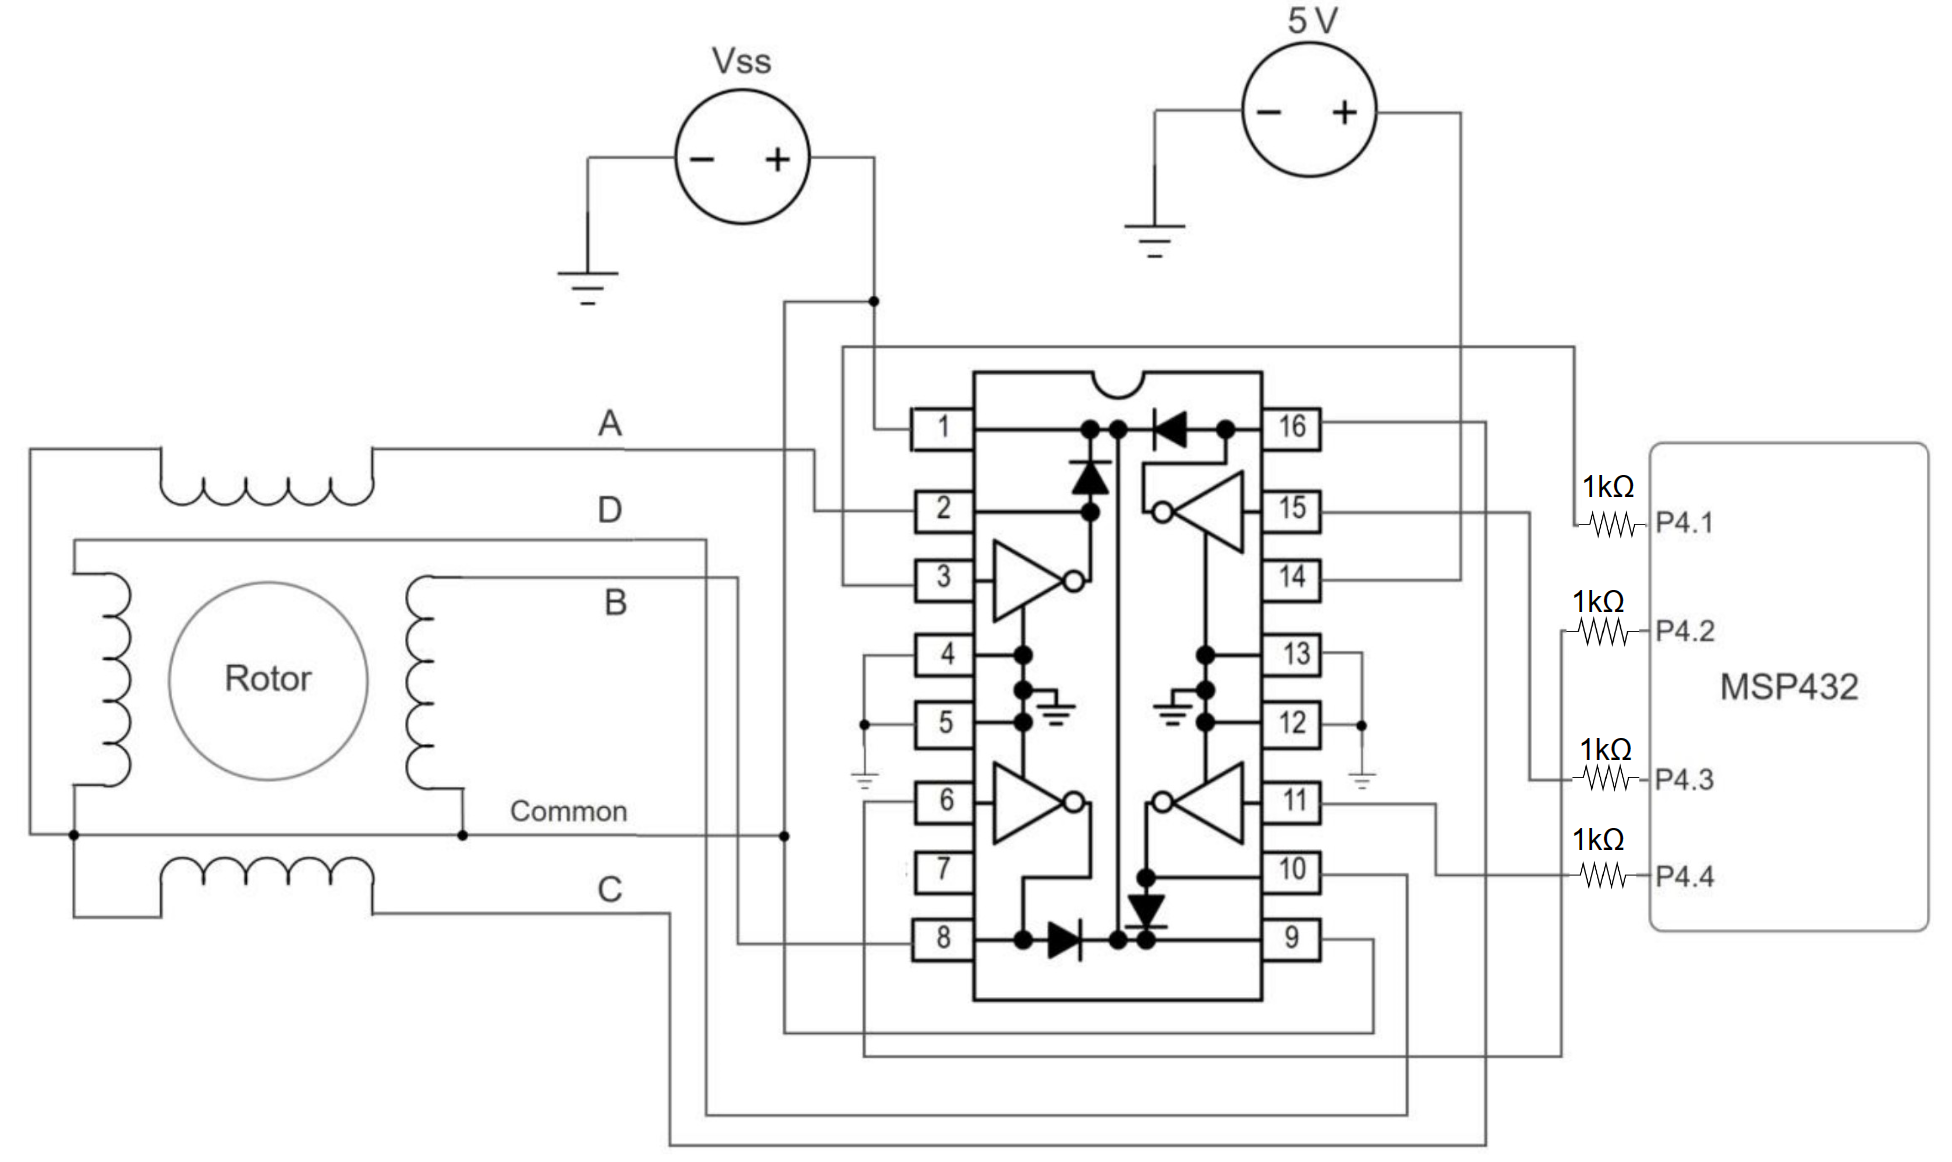
\includegraphics[width=0.75\textwidth]{StepperWiring.png}
    \caption{Stepper Motor Wiring}
    \label{fig:ServoWiring}
\end{figure}

\begin{figure}[H]
    \centering
    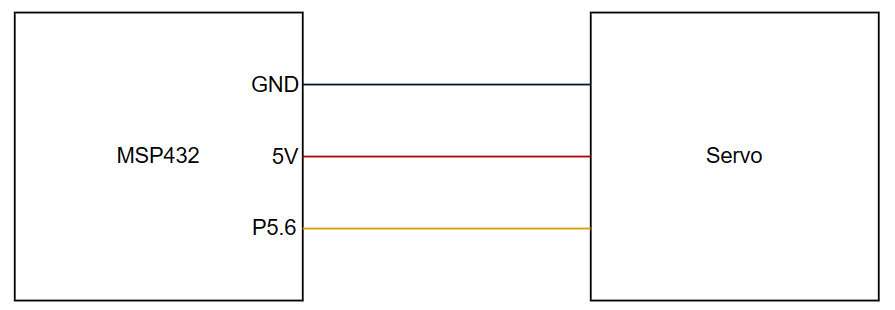
\includegraphics[width=0.75\textwidth]{ServoWiring.png}
    \caption{Servo Wiring}
    \label{fig:SevoWiring}
\end{figure}

\begin{figure}[H]
    \centering
    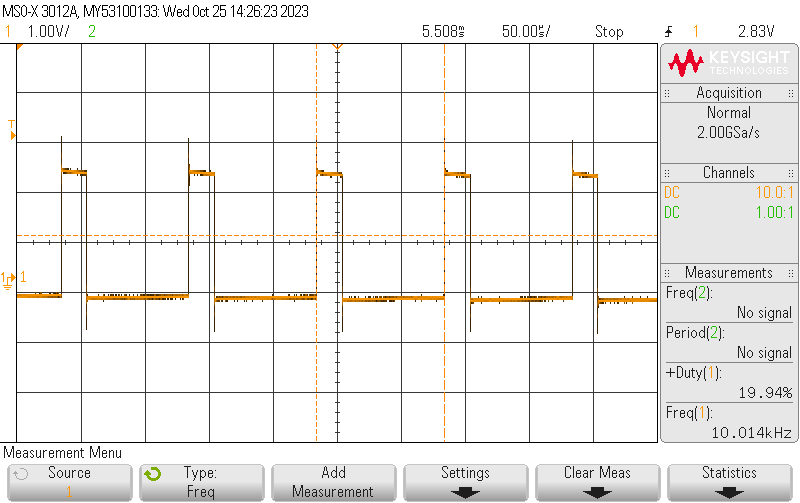
\includegraphics[width=0.75\textwidth]{PWM.png}
    \caption{PWM Waveform}
    \label{fig:pwm}
\end{figure}

\begin{figure}[H]
    \centering
    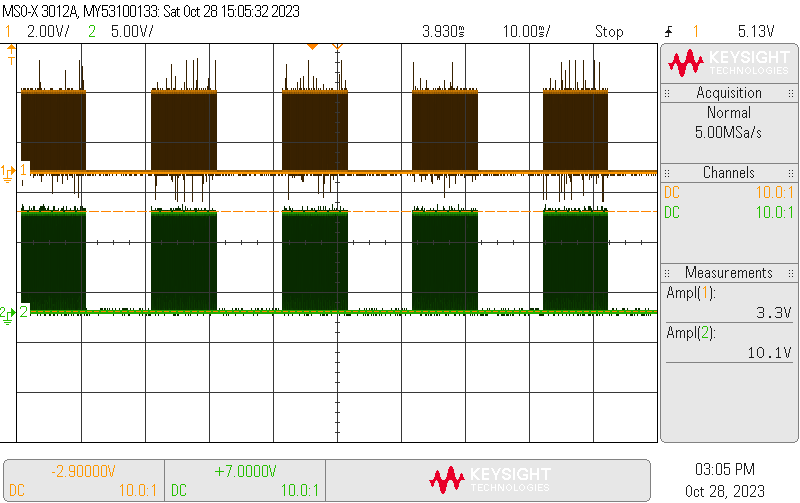
\includegraphics[width=0.75\textwidth]{MotorIO.png}
    \caption{Motor Input Output Waveform}
    \label{fig:motor}
\end{figure}

\begin{figure}[H]
    \centering
    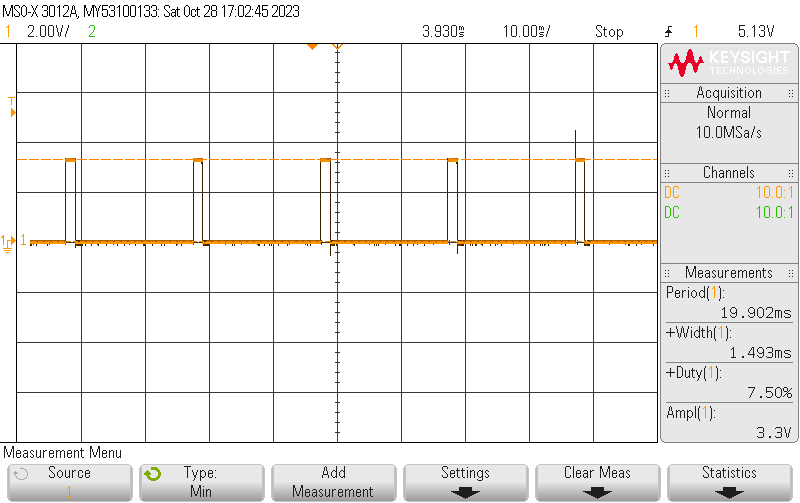
\includegraphics[width=0.75\textwidth]{ServoWave.png}
    \caption{Servo Input Waveform}
    \label{fig:ServoWave}
\end{figure}


\end{document}

